\chapter{Crystallisation}

In this chapter we apply the concepts of both dynamics and structure to investigate the dynamics of ordering. We use the dynamics from \textchapref{dynamics} to determine appropriate timescales for these events and the stable crystal structures and order parameters from \textchapref{structure} to identify regions of crystalline order.

\section{Melting Points}

In \textchapref{dynamics} we established the dynamics of our molecular systems which we can use to find the lowest temperature at which we expect to see crystallisation. To find the upper limit of crystallisation we need to identify the melting points of out molecules~\tabref{melting points}. From this data we can postulate the slow crystallisation we see in these molecules is a result of the large entropy difference between the liquid and crystal phases. This large entropy difference stabilises the liquid phase lowering the melting point such that the dynamics of the system are slow.

\begin{table}
    \centering
    \begin{tabular}{ | c  l | S S S S[table-format=2.2e+1] S[table-format=2.2e+1] |}
        \hline
        Molecule & Crystal & {Melting Point} & {$\Delta H$} & {$\Delta S$} & {$D$} & {$\tau_1$} \\ \hline
        \done & p2mg & 0.92 & 0.66 & 0.71 & 4.51e-6 & 1.03e3 \\
        \dcon & p2   & 1.90 & 0.95 & 0.50 & 1.09e-3 & 1.62e3 \\
        \tri  & p2   & 1.45 & 0.94 & 0.65 & 1.63e-4 & 4.54e3 \\
        \hline
    \end{tabular}
    \caption{Dynamic and thermodynamic properties at melting of the most stable crystal structures.}
    \label{tab:melting points}
\end{table}

The melting points were obtained from the analysis of two phase systems, where a central crystal region is surrounded by liquid. The temperature at which the size of the central crystal region begins to shrink are considered the melting point.

\section{Crystallisation Dynamics}

\subsection{Two Phase Systems}
\label{sec:two phase}

To get around the issues of waiting for a nucleation event to occur to see the growth of a crystal, we can create a two phase system in which the liquid-crystal boundary is already present. This can then be used to observe the growth of the crystal phase on this surface. Using these two phase configurations as the starting point we see crystallisation of the \done molecule~\figref{done crys}. It is interesting to note that the preferred crystal growth direction is at a \SI{45}{\degree} angle to the crystal boundary. Along with the crystal growth at the existing crystal interface there is also the nucleation of large crystals from the liquid, nucleation may be a fairly common event for the \done molecule.

\begin{figure}
    \begin{subfigure}{\textwidth}
        \includegraphics[width=\textwidth]{{{Snowman-0.75-0.637556-1.0-p2mg-1-frame-0000000000}}}
        \caption{}
        \label{fig:done p2mg init}
    \end{subfigure}
    \begin{subfigure}{\textwidth}
        \includegraphics[width=\textwidth]{{{Snowman-0.75-0.637556-1.0-p2mg-1-frame-0320000000}}}
        \caption{}
        \label{fig:done p2mg fine}
    \end{subfigure}
    \caption{The initial \subfigref{done p2mg init} and final \subfigref{done p2mg fine} configurations of a two phase system of the \done molecule containing the stable p2mg crystal in the center. The temperature is held at 0.75. Molecules considered crystalline are coloured according to their orientation such that antiparallel molecules have the same colour while non-crystalline molecules are grey. This system promotes growth at the boundary of the crystal as seen by the expanding region of teal colour.}
    \label{fig:done crys}
\end{figure}

The two phase analysis can also be performed on the \dcon system~\figref{dcon crys}. The order parameter we are using for the \dcon system appears to be less robust than for the \dcon system, \textfigref{dcon crys} shows many false negatives within the crystal system, while there are also more false positives, individual particles deemed as crystalline. However despite the noise in the order parameter we see growth of the crystal~\figref{dcon crys fine}, the regions where the ordered phase is lacking orientational order are regions of growth of the crystal. These orientationally disordered regions have to have come from the liquid phase as the crystal phase has all molecules in an antiparallel orientational order. Also like the \sone molecule we observe the spontaneous nucleation of ordered regions.

\begin{figure}
    \begin{subfigure}{\textwidth}
        \includegraphics[width=\textwidth]{{{Snowman-1.60-0.637556-1.637556-p2-1-frame-0000000000}}}
        \caption{}
        \label{fig:dcon crys init}
    \end{subfigure}
    \begin{subfigure}{\textwidth}
        \includegraphics[width=\textwidth]{{{Snowman-1.60-0.637556-1.637556-p2-1-frame-0320000000}}}
        \caption{}
        \label{fig:dcon crys fine}
    \end{subfigure}
    \caption{The initial \subfigref{dcon crys init} and final \subfigref{dcon crys fine} configurations of the two phase system of the \dcon molecule containing the favoured p2 crystal in the center. The temperature of this system is held at 1.60. Molecules considered ordered are coloured according to their orientation while molecule slacking order are grey. Growth of the crystal can be seen as coloured regions lacking the orientational order of the central crystalline region.}
    \label{fig:dcon crys}
\end{figure}

Unlike the \done and \dcon molecules the \tri molecules does not show crystallisation in the two phase system~\figref{tri crys}. The trimer shows small changes on the surface of the crystal between the initial~\figref{tri crys init} and the final~\figref{tri crys fine} configurations however these are more like what would occur at equilibrium, a rearrangement of the surface rather than growth, despite being below the melting point of the crystal phase. One explanation for this behaviour is the timescale that we are looking at is short compared to the rate of crystal growth.

\begin{figure}
    \begin{subfigure}{\textwidth}
        \includegraphics[width=\textwidth]{{{Trimer-1.30-0.637556-1.00-120-p2-1-frame-0000000000}}}
        \caption{}
        \label{fig:tri crys init}
    \end{subfigure}
    \begin{subfigure}{\textwidth}
        \includegraphics[width=\textwidth]{{{Trimer-1.30-0.637556-1.00-120-p2-1-frame-0320000000}}}
        \caption{}
        \label{fig:tri crys fine}
    \end{subfigure}
    \caption{The initial \subfigref{tri crys init} and final \subfigref{tri crys fine} of the two phase system of the \tri molecule with the favoured p2 crystal in the central region. The temperature of this system is held at 1.30. Molecules considered ordered are coloured according to their orientation such that molecules that are antiparallel are coloured the same while non-crystalline regions are grey. Despite being below the melting point of the crystal there is no significant net growth of the crystal phase.}
    \label{fig:tri crys}
\end{figure}

\subsection{Spontaneous Nucleation}

We have seen spontaneous nucleation from both the \done and \dcon molecules in the two phase system. We want to be able to see this nucleation from a random starting phase, to show that this is not just a remnant of order from the crystal the liquid phase was melted from. To see this nucleation we had to run simulations far longer than the simulations for dynamics.

The \done molecule shows significant regions of crystallinity~\figref{done nuc}. The configuration is dominated by a number of peach coloured crystals, the dominance of this orientation can be explained by examining the bottom right corner, between above the crystal there are layers of molecules with a more complex ordered structure, this structure forms most of the links between the peach crystal regions keeping them aligned. The other interesting feature of the crystal structure is the boundary between the lavender and peach~\cite{munroe:10} regions where the molecules alternate the crystal structure they are a part of, like a zipper connecting these two crystal regions.

\begin{figure}
    \includegraphics[width=\textwidth]{{{Snowman-0.75-0.637556-1.0-frame-2147000000}}}
    \caption{Configuration of the \done molecule showing significant crystal growth. Along with the p2mg crystal, coloured to show orientation such that antiparallel molecules have the same colour, there are regions of ordered structure not coloured.}
    \label{fig:done nuc}
\end{figure}

\begin{figure}
    \centering
    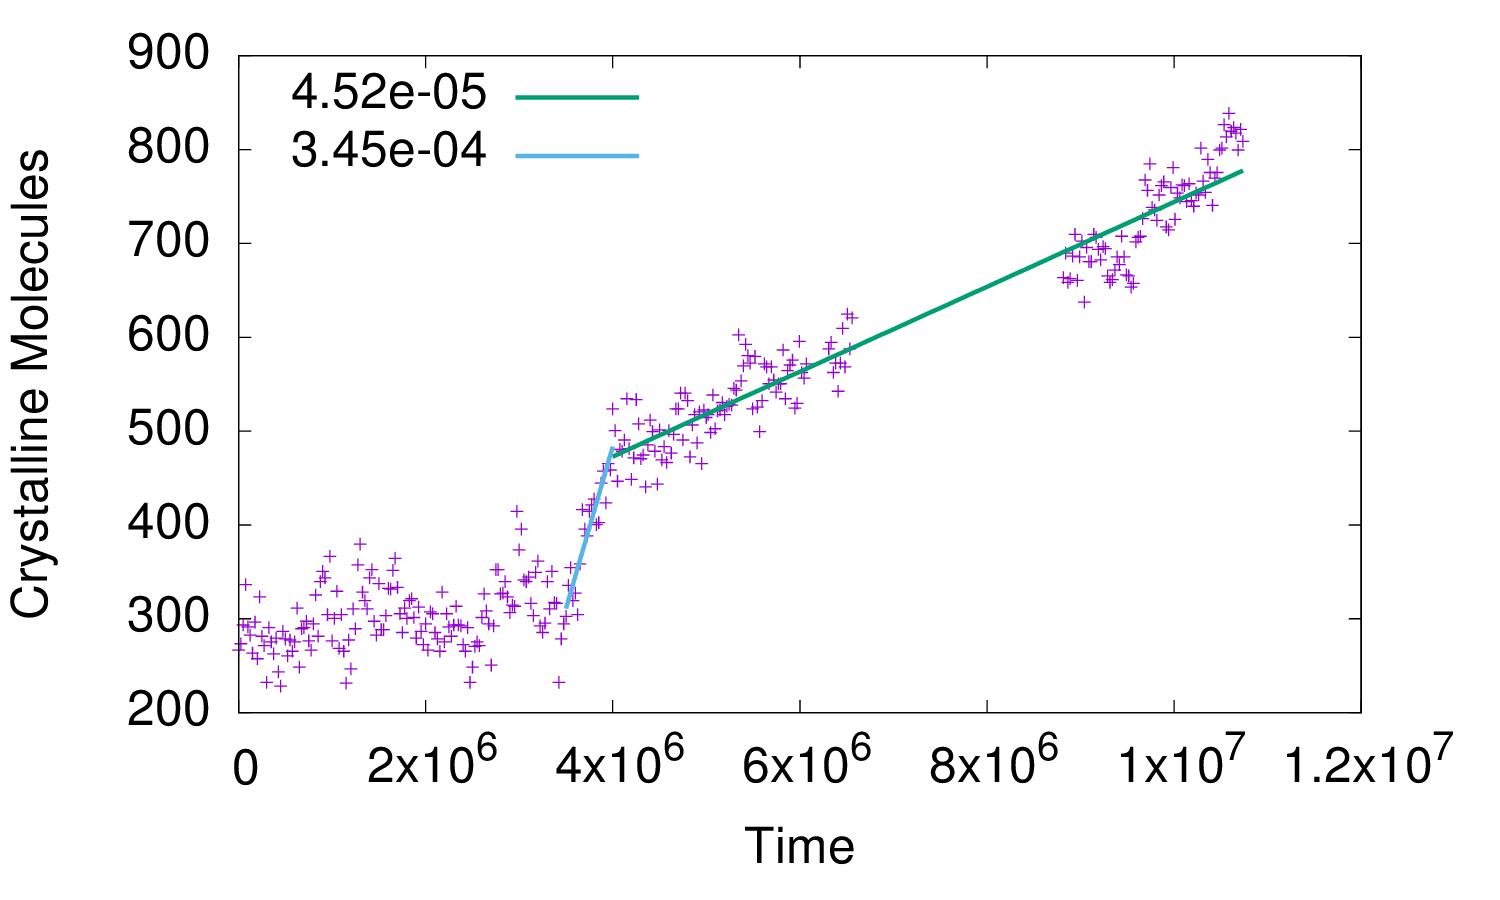
\includegraphics[width=0.7\textwidth]{done_crys_growth}
    \caption{Crystal growth of the \done molecule counting the number of molecules considered crystalline in each configuration. The region of crystal growth (green) has a growth rate of \num{4.52e-5} molecules per unit time with the nucleation rate (blue) of \num{3.45e-4} molecules per unit time.}
\end{figure}

Measuring the crystal growth rate we can compare this to the dynamics of the system at these temperatures, at a temperature of 0.75 the \done molecule has a structural relaxation time of \num{4.3e5} an order of magnitude smaller than the time before the nucleation event. However the large nucleation event occurred on the timescale of a structural relaxation; crystallisation in the \done molecule can occur with very small motions of molecules.
